\documentclass{article}
\usepackage[utf8]{inputenc}
\usepackage{amsmath}
\usepackage{indentfirst}
\usepackage{graphicx,caption}
\usepackage[a4paper, margin=1in]{geometry}
\linespread{1.15}
\usepackage{empheq}
\usepackage[most]{tcolorbox}
\usepackage[margin=3cm]{caption}
\usepackage{siunitx}
\usepackage{array}
\usepackage{braket}
\usepackage{mathtools}

\usepackage{xcolor,sectsty}
\definecolor{astral}{RGB}{46,116,181}
\subsectionfont{\color{astral}}
\sectionfont{\color{astral}}

\title{
\includegraphics[width=0.1\textwidth]{ufallogo.png} \\
\Huge{\color{astral}\textbf{Informação Quântica}}}
\author{Paulo Brandão}
\date{Maio de 2017}

\newtcbox{\mymath}[1][]{%
    nobeforeafter, math upper, tcbox raise base,
    enhanced, colframe=blue!30!black,
    colback=blue!30, boxrule=1pt,
    #1}
\newcommand*{\bfrac}[2]{\genfrac{\lbrace}{\rbrace}{0pt}{}{#1}{#2}}
\begin{document}

\maketitle

\section{Introdução}

A ciência da teoria da informação começa com o reconhecimento de que existe uma ligação fundamental entre probabilidade e informação. Logo no começo do século 18, Bayes sabia que probabilidades dependem do que conhecemos. Se adquirimos uma informação adicional então isso modifica a probabilidade. Que a probabilidade é um conceito relativo à informação que alguém possui é fácil de ver. Suponha que Bob coloque um prêmio dentro de uma de três caixas disponíveis e peça para que Alice escolha uma das caixas. Se ela acertar, ganha o prêmio. Nesse simples exemplo é fácil ver que a probabilidade de acerto para Bob é 1 (ele sabe em qual caixa está o prêmio!) e 1/3 para Alice. Assim, probabilidade depende da informação na qual o indivíduo possui.

Informação é uma função das probabilidades: ela é a entropia associada à distribuição de probabilidades. A grande descoberta da entropia como uma quantidade de informação foi revelada por Shannon na sua teoria matemática da comunicação (clássica) em 1948. O trabalho de Shannon envolveu, além da visão probabilística para a informação, dois teoremas extremamente importantes que mostram a limitação imposta em qualquer sistema para transmitir informação.

A conexão entre probabilidade e informação têm aplicações muito mais amplas do que apenas comunicação. De fato, podemos esperar que as ideias da teoria da comunicação se apliquem em quaisquer sistemas que sejam de natureza estatística ou probabilística. A mecânica quântica é, por natureza, uma teoria probabilística e então era de se esperar que uma teoria quântica da informação fosse desenvolvida. Curiosamente, apesar do grande avanço dos últimos anos, ainda não se obteve uma teoria quântica da informação completa, fechada, como a teoria clássica. A teoria quântica da informação combina aspectos da teoria clássica da informação com as leis da mecânica quântica e, por essa razão, é esperado que informação quântica se comporte de uma maneira bem diferente da sua contraparte clássica. E isso é realmente o que acontece, como iremos ver no decorrer da aula.

O objetivo dessa aula é apresentar ao estudante os conceitos primordiais das teorias clássica e quântica da informação no contexto da transmissão de estados clássicos e quânticos. A área de pesquisa em informação quântica é extremamente vasta e será impossível tratar de todos os seus aspectos em uma única aula. Assim,  



\section{Informação clássica e a entropia de Shannon}

Antes de desenvolver a teoria quântica da informação no contexto da transmissão de dados, é útil descrever os aspectos mais básicos da teoria clássica da informação, desenvolvidos por Shannon. O motivo disso é que várias quantidades são definidas de forma bastante semelhantes nos dois casos. Além disso, como o estudante geralmente não tem um encontro com os básicos da teoria clássica da informação, é vantajoso, e muito gratificante, conhecer o trabalho que Claude Shannon desenvolveu na década de 40. Vamos começar a discussão com um exemplo muito simples de transmissão de informação que nos ajudará a definir informação de uma maneira quantitativa.

Suponha que Alice queira informar seu estado de espírito para seu namorado Bob que se encontra muito distante. Ela utiliza quatro símbolos para representar os quatro estados, como indica a tabela abaixo:
\begin{center}
\begin{tabular}{ |c|c|c| } 
\hline
Símbolo & Significado \\
\hline
$A$ & ``Estou triste''  \\ 
$B$ & ``Estou com raiva'' \\ 
$C$ & ``Estou feliz'' \\
$D$ & ``Estou com tédio'' \\
\hline
\end{tabular}
\end{center}
Bob é um cara muito paciente e conta quantas vezes recebeu cada símbolo num total de $N$ vezes consecutivas. Ele conclui que
\begin{center}
    $A$ apareceu $N_A$ vezes; \\
    $B$ apareceu $N_B$ vezes; \\
    $C$ apareceu $N_C$ vezes; \\
    $D$ apareceu $N_D$ vezes. \\
\end{center}
Temos claro que $N_A + N_B + N_C + N_D = N$. Assim, Bob, que conhece um pouco as leis da probabilidade, associa uma probabilidade para cada estado de Alice:
\begin{center}
    $A$ $\rightarrow$ $p(A) = N_A/N$; \\
    $B$ $\rightarrow$ $p(B) = N_B/N$; \\
    $C$ $\rightarrow$ $p(C) = N_C/N$; \\
    $D$ $\rightarrow$ $p(D) = N_D/N$. \\
\end{center}
Vamos ilustrar algumas situações possíveis com 3 casos.
\begin{itemize}
    \item Caso 1: Alice está sempre feliz.
\end{itemize}
Neste caso, a probabilidade de Bob receber o estado $C$ é 1, como indica a Figura 1. É fácil ver que Bob não ganha nenhuma informação nessa situação. Se alguém perguntar a ele como está Alice, ele irá responder que ela está certamente feliz. Não há dúvidas sobre o estado de Alice e cada vez que Bob recebe a mensagem ele não conclui nada de novo. Isto é, não há informação nova. Em termos mais precisos dizemos que o \textbf{conteúdo informativo da mensagem é nulo}.

\begin{figure}[h]
\centering
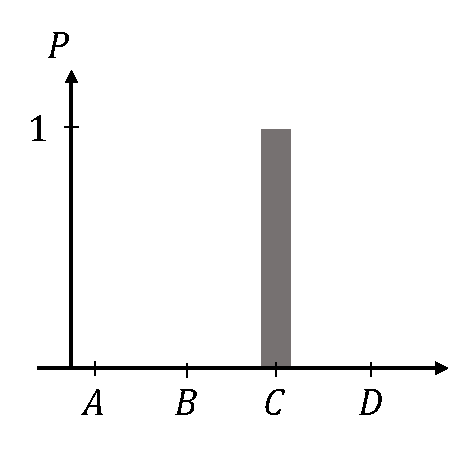
\includegraphics[width=4cm]{caso1.pdf}
\captionsetup{labelsep=none}
\caption{. Distribuição de probabilidades quando $p(C) = 1$ e todos os outros estados são nulos. Alice está sempre feliz. Como o estado de Alice é conhecido com 100\% de certeza, o conteúdo informativo da mensagem é nulo. }
\end{figure}
\newpage 
\begin{itemize}
    \item Caso 2: O estado de Alice muda aleatoriamente.
\end{itemize}
Neste caso, o estado de alice muda de uma maneira completamente aleatória, como indica a distribuição de probabilidades da Figura 2. Em certas ocasiões Alice estará feliz, em outras com raiva, etc. Se alguém perguntar para Bob sobre o estado de Alice, ele certamente não conseguirá descrever para a pessoa. Cada vez que Bob recebe uma mensagem nova, ele ganha uma informação sobre o estado atual de Alice. Isto é, há uma informação na mensagem descrita pela distribuição de probabilidades da Figura 2. Em termos mais precisos dizemos que há um conteúdo informativo na mensagem.
\begin{figure}[h]
\centering
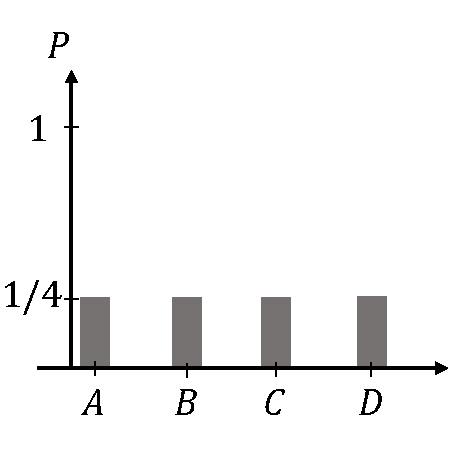
\includegraphics[width=4cm]{caso2.pdf}
\captionsetup{labelsep=none}
\caption{. Distribuição de probabilidades quando $p(A) = p(B) = p(C) = p(D) = 1/4$. O estado de Alice muda aleatoriamente. Nesta situação, cada vez que Bob recebe uma mensagem, adquire uma informação nova. }
\end{figure}

\begin{itemize}
    \item Caso 3: Os estados de alice tem probabilidades diferentes.
\end{itemize}
Nesta situação, Alice tem mais chances de estar triste, pois $p(A) = 1/2$, do que estar com raiva, $p(B) = 1/4$, ou feliz e com tédio, $p(C) = p(D) = 1/8$. Dessa forma, é provável que Bob espere, após várias mensagens trocadas, que Alice esteja triste na média. No entanto, como os estados ainda são aleatórios, Bob ainda ganha informação sobre cada mensagem recebida. O conteúdo informativo é, claro, menor que o conteúdo informativo do Caso 2 e maior que o conteúdo informativo do Caso 1.

\begin{figure}[h]
\centering
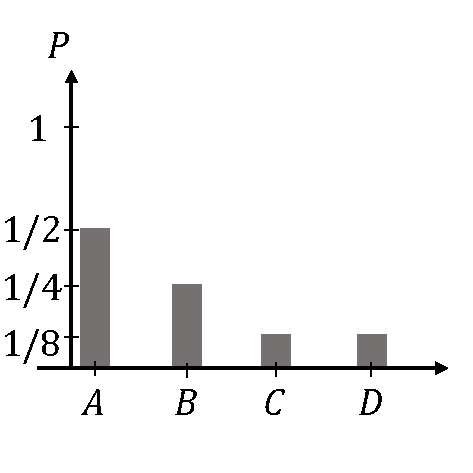
\includegraphics[width=4cm]{caso3.pdf}
\captionsetup{labelsep=none}
\caption{. Distribuição de probabilidades quando $p(A) = 1/2$, $p(B) = 1/4$ e $p(C) = p(D) = 1/8$. O estado de Alice muda a cada mensagem mas com as probabilidades diferentes (apenas $C$ e $D$ são iguais). Neste caso, o conteúdo informativo da mensagem é maior que o Caso 1 e menor que o Caso 2. }
\end{figure}

Encontramos dessa forma uma conexão profunda entre \textbf{incerteza e informação}. Quanto mais incerto é o resultado, mais informação Bob ganha. A distribuição uniforme (Caso 2) representa a situação onde Bob está mais incerto acerca do estado de Alice, assim seu conteúdo informativo é máximo. A primeira grande ideia de Shannon foi quantificar o conteúdo informativo de uma mensagem através da \textbf{entropia de Shannon}:
\begin{equation}
    H_S = - \sum_i p_i \log_2 p_i \hspace{0.2cm} \text{(bits)},
\end{equation}
onde $p_i$ representa a probabilidade do evento $i$ acontecer e definimos o logaritmo na base 2. Dessa forma, a entropia é medida em bits. Fica como exercício para o estudante (ver lista de exercícios) mostrar que $H_S \geq 0$. É fácil ver que a entropia de Shannon caracteriza o conteúdo informativo de uma mensagem descrita pelas probabilidades $p_i$. Vamos aplicá-la na comunicação existente entre Alice e Bob. No Caso 1 temos
\begin{equation}
\begin{split}
    H_S &= -p(A)\log_2 p(A) - p(B)\log_2 p(B)-p(C)\log_2 p(C)-p(D)\log_2 p(D) \\
        &= -0 \cdot \log_2 0 -0 \cdot \log_2 0 - 1 \cdot \log_2 1 -0 \cdot \log_2 0 \\
        &= 0 \text{ bits},
\end{split}
\end{equation}
onde assumimos que $0\cdot\log_2 0 = 0$. Como esperado, o conteúdo informativo da primeira mensagem, onde Alice diz somente que está feliz, é zero. Não há informação adquirida por Bob nessa comunicação (ele já sabe o que esperar). No segundo caso, a distribuição de probabilidades é uniforme e o conteúdo informativo da mensagem vale
\begin{equation}
\begin{split}
    H_S &= -p(A)\log_2 p(A) - p(B)\log_2 p(B)-p(C)\log_2 p(C)-p(D)\log_2 p(D) \\
        &= -(1/4) \cdot \log_2 (1/4) -(1/4) \cdot \log_2 (1/4) - (1/4) \cdot \log_2 (1/4) -(1/4) \cdot \log_2 (1/4) \\
        &= 2 \text{ bits},
\end{split}
\end{equation}
que não é nulo, como esperado. Assim, na segunda situação, Bob ganha uma informação. O número dois indica simplesmente que, \textbf{para essa distribuição de probabilidades}, dois bits são necessários por cada caractere a ser transmitido. Iremos discutir esse ponto mais a frente. Para o Caso 3 o estudante pode demonstrar através dos exemplos anteriores que $H_S = 7/4 = 1,75$ bits. Como esperado, esse valor do conteúdo informativo é maior que o Caso 1 e menor que o Caso 2. Em resumo:
\begin{empheq}[box=\tcbhighmath]{equation}
\text{\textbf{Maior entropia}} \Longrightarrow \text{\textbf{Mais informação}}
\end{empheq}


Após Shannon quantificar o conteúdo informativo de uma mensagem através da entropia $H_S$, ele estudou a maneira de como podemos transmitir informação de uma fonte para um receptor. A teoria matemática da comunicação, desenvolvida por Shannon, é estruturada em torno de dois teoremas muito importantes. Ambos utilizam a ideia da compressão de uma mensagem. Vamos supor que Alice transmite seu estado uma vez por dia. Durante o período de 1 semana, Bob recebeu a seguinte sequêcia de caracteres
\begin{center}
    $DBAACAA$
\end{center}
O sistema de transmissão, entretanto, não envia os caracteres $A$ ou $D$, e sim sinais analógicos ou digitais. A maneira mais simples de codificar os caracteres $\{ A,B,C,D \}$ nessa linguagem é utilizar a base binária onde podemos associar
\begin{center}
    $A \Longrightarrow 00$ \hspace{0.5cm} $B \Longrightarrow 01$
\end{center}
\begin{center}
    $C \Longrightarrow 10$ \hspace{0.5cm} $D \Longrightarrow 11$
\end{center}
Assim, a mensagem acima para os caracteres seria codificada na base binária resultando na sequência
\begin{equation}
    11010000100000
\end{equation}
Note que não há ambiguidades na mensagem codificada. Qualquer sequência de caracteres pode ser unicamente representada na forma binária. Shannon se perguntou se não seria possível utilizar um conjunto menor de bits para representar a mesma mensagem a ser transmitida por um canal de comunicação \textbf{sem ruído}. O adjetivo ``sem ruído'' implica que se Alice envia o estado $A$ então Bob recebe o estado $A$ e assim para os outros estados disponíveis. Em palavras, o meio por onde ocorre a transmissão de informação não pode mudar os estados transmitidos, o que é sempre uma aproximação na prática. Shannon estava interessado em excluir as redundâncias associadas à mensagem e do ponto de vista prático, esse é um tema muito importante porque quanto menor for a mensagem codificada, menos caracteres poderão ser transmitidos pelo canal de comunicação. Curiosamente, a resposta para essa pergunta é dada pela entropia de Shannon $H_S$! \textbf{Ela representa o número médio de bits necessários por caractere}. Esse resultado é conhecimento como \textbf{teorema da codificação sem ruído de Shannon}. Sem compressão, a mensagem $DBAACAA$ pode ser transmitida como mostra a sequência binária acima, e de fato essa é a maneira mais otimizada se a distribuição de probabilidades dos caracteres for uniforme, como no Caso 2 discutido anteriormente. No entanto, se a distribuição $p_i$ não for uniforme, podemos utilizar esse fato para representar os caracteres mais prováveis por menos bits e os menos prováveis por mais bits, de modo a obter um número de bits menores na média. Por exemplo, se a distribuição de probabilidades dos caracteres for a mesma que no Caso 3, podemos associar
\begin{center}
    $A \Longrightarrow 0$ $[p(A) = 1/2]$ \hspace{0.5cm} $B \Longrightarrow 10$ $[p(B) = 1/4]$
\end{center}
\begin{center}
    $C \Longrightarrow 110$ $[p(C) = 1/8]$ \hspace{0.5cm} $D \Longrightarrow 111$ $[p(C) = 1/8]$
\end{center}
de modo que a mesma mensagem pode ser codificada pela sequência binária 
\begin{equation}
    111100011000
\end{equation}
que contém um número menor de bits que a sequência (5). O comprimento médio da sequência pode ser calculado como
\begin{equation}
    \text{Para a sequência de bits (5): } \frac{1}{2}\cdot 2 + \frac{1}{2}\cdot 2 + \frac{1}{2}\cdot 2 + \frac{1}{2}\cdot 2 = 2 = H_S
\end{equation}
\begin{equation}
    \text{Para a sequência de bits (6): } \frac{1}{2}\cdot 1 + \frac{1}{4}\cdot 2 + \frac{1}{8}\cdot 3 + \frac{1}{8}\cdot 3 = 7/4 = H_S
\end{equation}
cujo valor numérico é o mesmo calculado utilizando a entropia de Shannon. É fácil ver, portanto, que a entropia de Shannon nos dá o número médio de bits por caractere necessário para transmitir a mensagem através de um canal sem ruído de modo a não se perder informação. Qualquer compressão da mensagem que vá além do permitido pela entropia de Shannon irá, inevitavelmente, fazer com que a mensagem seja transmitida com erros. A única sutileza por trás da teoria da comunicação de Shannon é que esse resultado só é válido quando o número de caracteres é muito grande $N \rightarrow \infty$.

O outro teorema de Shannon envolve assumir que o sistema por onde a mensagem é transmitida afeta a mensagem de tal forma que bits possam ser trocados de uma maneira fundamental que não controlamos. Obviamente essa situação não é desejada mas, infelizmente, está sempre presente na vida prática. Shannon, entretanto, demonstrou que ainda é possível representar uma sequência de $N$ bits de uma mensagem comprimida e transmiti-la pelo canal com ruído de forma que o receptor ainda consiga recuperar a mensagem completa. É fácil de perceber também que essa situação é mais complicada de se tratar quantitativamente e vai além do nível desta aula. Entretanto, para o aluno que quiser estudar esses temas mais a fundo, pode consultar a lista de referências no plano de aula. Esses dois teoremas formam a base da teoria da informação clássica desenvolvida por Shannon e são aplicados diariamente em inúmeras situações do cotidiano.


\section{Informação quântica e a entropia de von Neumann}


Vamos supor agora que Alice tenha em posse apenas dois estados quânticos ortogonais, $\ket{0}$ e $\ket{1}$, chamados de \textit{qubits}. Se a transmissão fosse por canais clássicos seguindo as regras da física clássica, Alice poderia transmitir apenas $\ket{0}$ ou $\ket{1}$ com determinadas probabilidades, assim como ela transmitiu $A$, $B$, $C$ e $D$ na seção anterior. No entanto, a mecânica quântica é muito diferente da mecânica clássica na descrição de seus estados. Na teoria quântica é possível criar um novo estado a partir da \textit{superposição quântica}. Essa possibilidade extra fornecida pela descrição quântica faz com que informação quântica possua características e comportamentos bastantes distintos da sua contraparte clássica, como veremos nesta seção.

Alice pode transmitir para Bob uma sequência de $n$ estados quânticos
\begin{equation}
    \{ \ket{w_1},\ket{w_2},...,\ket{w_n} \}
\end{equation}
com respectivas probabilidades
\begin{equation}
    \{ p_1, p_2, ..., p_n \},
\end{equation}
onde cada $\ket{w_i}$ pode ser escrito como uma superposição dos qubits fundamentais $\ket{0}$ e $\ket{1}$ e $p_1 + p_2 + ... + p_n = 1$. Por exemplo, Alice pode escolher transmitir os três estados (que não precisam ser ortogonais)
\begin{equation}
    \ket{w_1} = \ket{1}, \hspace{0.5cm}
    \ket{w_2} = \frac{1}{\sqrt{2}}\ket{0} + \frac{1}{\sqrt{2}}\ket{1}, \hspace{0.5cm}
    \ket{w_3} = \frac{\sqrt{3}}{2}\ket{0} + \frac{1}{2}\ket{1}
\end{equation}
com as respectivas probabilidades
\begin{equation}
    p_1 = p(\ket{w_1}) = 1/2, \hspace{0.5cm} p_2 = p(\ket{w_2}) = 1/4, \hspace{0.5cm} p_3 = p(\ket{w_3}) = 1/4.
\end{equation}
Assim, Bob receberá uma sequência de estados com determinadas probabilidades, análogo ao caso clássico, e deverá efetuar uma medida em cada estado recebido. Uma maneira mais elegante e útil de caracterizar os estados de Alice e  suas probabilidades é através do operador densidade da fonte $\hat{\rho}$. O operador densidade pode ser escrito de forma geral
\begin{equation}
    \hat{\rho} = p_1\ket{w_1}\bra{w_1} + p_2\ket{w_2}\bra{w_2} + ... + p_n\ket{w_n}\bra{w_n} = \sum_{i=1}^n p_i \ket{w_i}\bra{w_i}
\end{equation}
onde, mais uma vez, os estados $\ket{w_i}$ não precisam ser ortogonais. Para o exemplo considerado acima, podemos escrever
\begin{equation}
\begin{split}
    \hat{\rho} &= p_1\ket{w_1}\bra{w_1} + p_2\ket{w_2}\bra{w_2} + p_3\ket{w_3}\bra{w_3} \\
               &= \frac{1}{2}\ket{1}\bra{1} + \frac{1}{8}\left( \ket{0} + \ket{1} \right)\left( \bra{0} + \bra{1} \right) + \frac{1}{16}\left( \sqrt{3}\ket{0} + \ket{1} \right)\left( \sqrt{3}\bra{0} + \bra{1} \right) \\
               &= \frac{5}{16}\ket{0}\bra{0} + \frac{2+\sqrt{3}}{16}\ket{0}\bra{1}+ \frac{2+\sqrt{3}}{16}\ket{1}\bra{0} + \frac{11}{16}\ket{1}\bra{1} \\
               &= \rho_{00}\ket{0}\bra{0} + \rho_{01}\ket{0}\bra{1}+ \rho_{10}\ket{1}\bra{0} + \rho_{11}\ket{1}\bra{1},
\end{split}
\end{equation}
onde $\rho_{ij} = \braket{i|\hat{\rho}|j}$ representam os elementos da matriz densidade na base padrão de qubits. Bob precisa fazer a medida dos estados recebidos. Mas o que é uma medida em mecânica quântica? É simplesmente uma projeção do estado recebido em algum outro estado. Assim, Bob precisa, antes de tudo, escolher um conjunto de kets no qual ele quer efetuar as medidas. Ele pode, por exemplo, escolher medir os estados recebidos na base padrão $\ket{0}$ e $\ket{1}$. Se Alice envia o estado $\ket{w_1}$, boba mede esse estado fazendo o produto interno $\braket{1|w_1}$






\end{document}
